\subsection{Configuración de Bacula en Debian}

\textbf{Configuración del Firewall}
\medskip

Primero, es necesario añadir las reglas al firewall para permitir el tráfico en los puertos utilizados por los componentes de Bacula. Los puertos son 9101 para el Director, 9102 para el File Daemon y 9103 para el Storage Daemon. Usamos los siguientes comandos:
\begin{verbatim}
sudo ufw allow 9101/tcp
sudo ufw allow 9102/tcp
sudo ufw allow 9103/tcp
\end{verbatim}

\begin{figure}[H]
    \centering
    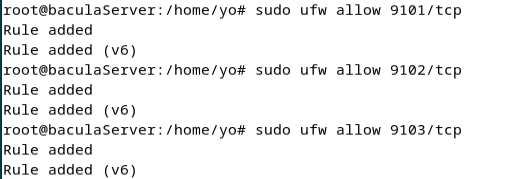
\includegraphics[width=0.5\linewidth]{instalacionBacula/puertosBaCULAufw.png}
    \caption{Adición de reglas al firewall para Bacula}
\end{figure}

\textbf{Acceso a los Repositorios de Bacula}\medskip

Para instalar Bacula, primero debemos tener acceso a los repositorios. Es necesario registrarse en la página oficial \url{https://www.bacula.org/} para acceder a los repositorios de Bacula.

\begin{figure}[H]
    \centering
    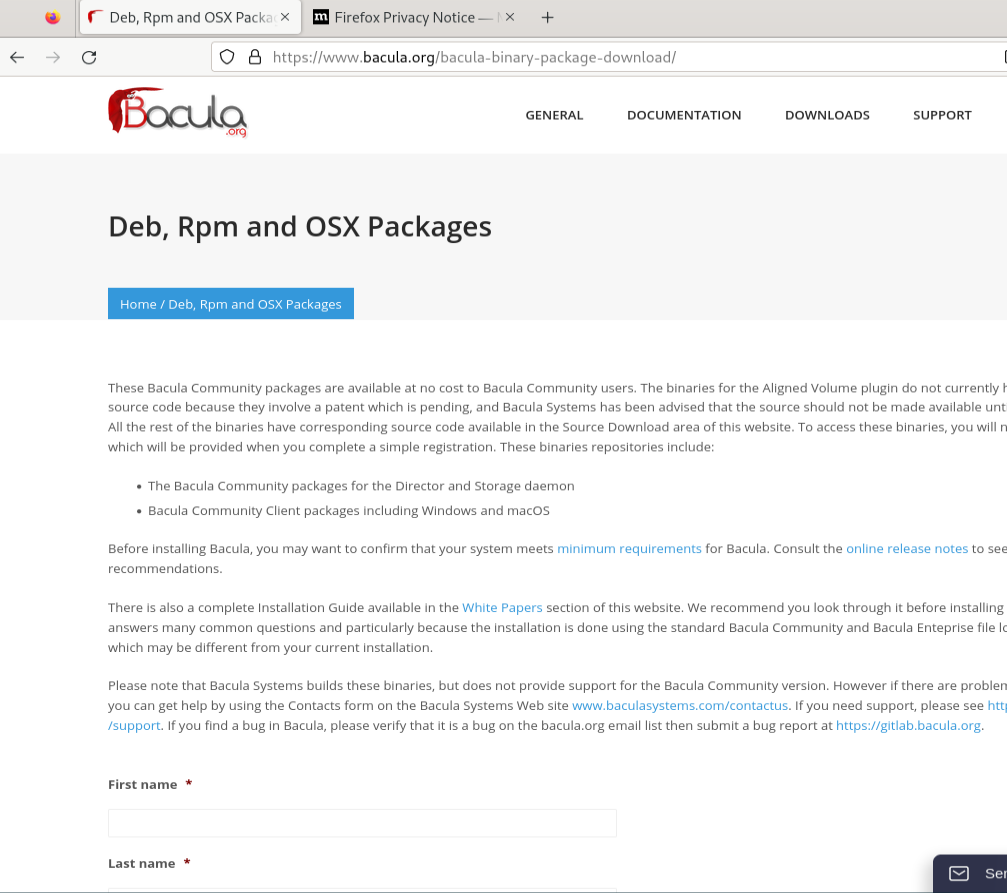
\includegraphics[width=0.5\linewidth]{instalacionBacula/registroBacula.png}
    \caption{Página de registro para acceso a repositorios de Bacula}
\end{figure}

\textbf{Descarga e Instalación de Bacula}\medskip

Una vez registrados, accedemos a la sección de binarios y seleccionamos la última versión disponible para nuestro sistema.

\begin{figure}[H]
    \centering
    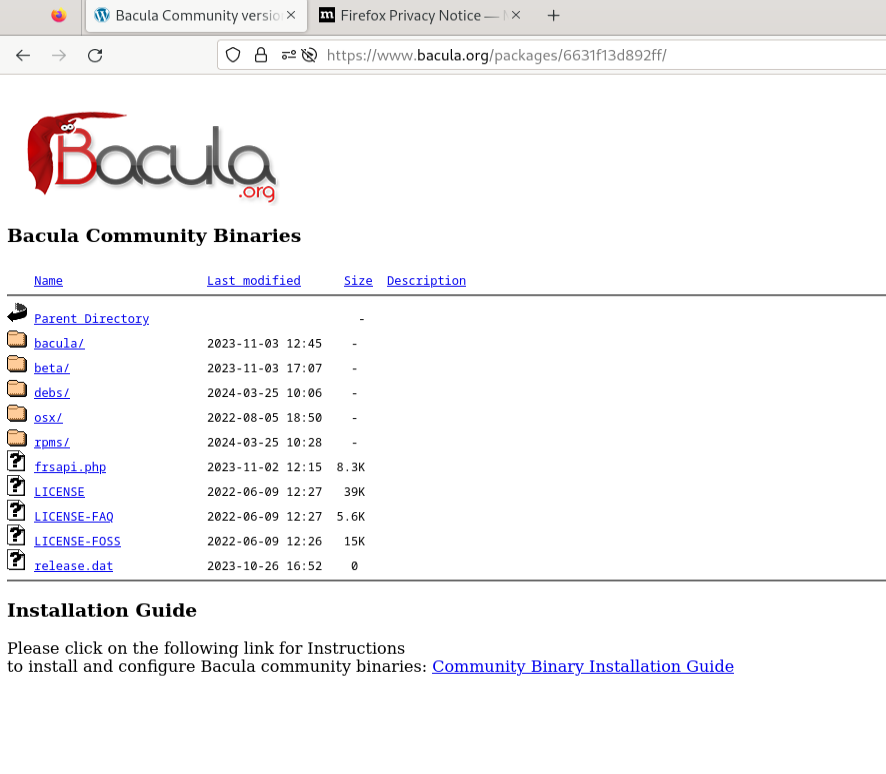
\includegraphics[width=0.5\linewidth]{instalacionBacula/baculapackages.png}
    \caption{Acceso a los binarios de Bacula}
\end{figure}

\textbf{Añadir Clave de Verificación y Repositorio}\medskip

Añadimos la clave de verificación y el repositorio de Bacula a nuestro sistema con los siguientes comandos:
\begin{verbatim}
wget https://bacula.org/downloads/Bacula-4096-Distribution-Verification-key.asc
apt-key add Bacula-4096-Distribution-Verification-key.asc
\end{verbatim}

\begin{figure}[H]
    \centering
    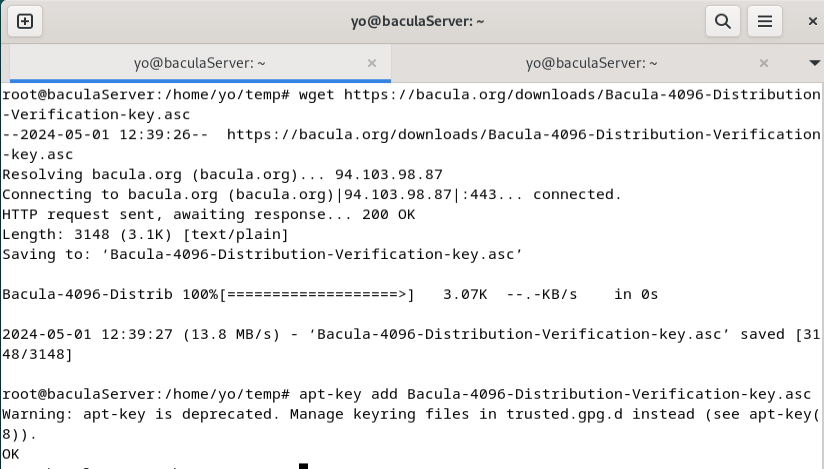
\includegraphics[width=0.5\linewidth]{instalacionBacula/baculaSignature.png}
    \caption{Añadiendo la clave de verificación de Bacula}
\end{figure}

\begin{figure}[H]
    \centering
    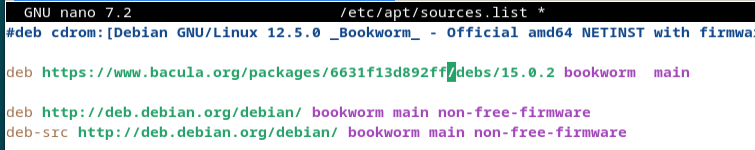
\includegraphics[width=0.5\linewidth]{instalacionBacula/baculaRepositorio.png}
    \caption{Añadiendo el repositorio de Bacula a sources.list}
\end{figure}

\textbf{MySQl vs PostgreSQL}
\medskip

Antes de seguir un aspecto importante es que base de datos para el catalogo elegir.


Cuando configuras Bacula para gestionar copias de seguridad, elegir entre MySQL y PostgreSQL para su servicio de catálogo puede depender de varias consideraciones técnicas y de licencia. A continuación, se presenta una comparación detallada:



\begin{table}[H]
    \centering
    \small
    \begin{tabularx}{\textwidth}{>{\centering\arraybackslash}p{0.15\textwidth}>{\centering\arraybackslash}p{0.4\textwidth}>{\centering\arraybackslash}X} 
        \hline
        \thead{Aspecto} & \thead{MySQL} & \thead{PostgreSQL} \\
        \hline
        Licencia & GNU GPL, que es más restrictiva en términos de obligaciones de compartir cambios & BSD, más permisiva y flexible para el uso en productos derivados sin compartir el código.\\
        Madurez & Muy maduro y ampliamente adoptado en aplicaciones web y de empresa. & Extremadamente maduro, con un enfoque en características avanzadas y conformidad con SQL.\\
        Desempeño & Generalmente más rápido en operaciones de lectura y carga de trabajo menos complejas. & Excelente en transacciones complejas y operaciones concurrentes de alta integridad.\\
        Características & 	Orientado al rendimiento con características de usabilidad fácil. &Soporta un conjunto más amplio de características SQL, funciones avanzadas y tipos de datos. \\
        Soporte de Datos	& Bueno para manejar grandes volúmenes de datos en sitios menos complejos. & Mejor para manejar complejidades en grandes bases de datos y con requerimientos estrictos. \\
        Seguridad y Confiabilidad & Confiabilidad alta, pero PostgreSQL tiene una reputación superior en robustez y seguridad. & Considerado muy robusto y seguro, con soporte extenso para políticas de seguridad detalladas.\\
        Facilidad de Configuración & Relativamente fácil de configurar y popular en la comunidad con muchos recursos disponibles. & Requiere más configuración inicial pero es altamente personalizable.\\
        \bottomrule
    \end{tabularx}
    \caption{Comparación entre Postgresql y MySQL para el catálogo de bacula.}
\end{table}




Recomendaciones para usar MySQL o PostgreSQL con Bacula:

\begin{itemize}
    \item MySQL: Ideal para entornos donde la velocidad y la simplicidad son prioritarias. Su licencia GPL puede ser adecuada si el proyecto también se distribuirá bajo GPL o cuando la licencia no representa un problema.
    \item PostgreSQL: La mejor opción si se requiere un sistema de gestión de base de datos robusto, con características avanzadas y mejor conformidad con SQL. Su licencia BSD es favorable para incorporar Bacula en productos que no desean estar ligados a las restricciones de GPL.
\end{itemize}



\textbf{Instalación de Bacula con PostgreSQL}\medskip

Seleccionamos PostgreSQL como la base de datos para el catálogo de Bacula. Instalamos la base de datos y Bacula con los siguientes comandos:
\begin{verbatim}
apt-get install dbconfig-common postgresql
apt-get install bacula-postgresql
\end{verbatim}

\begin{figure}[H]
    \centering
    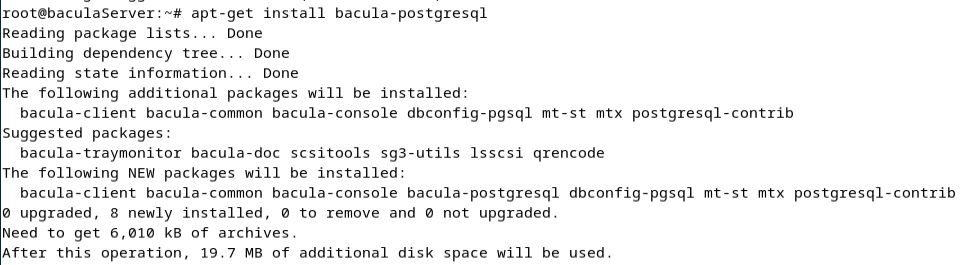
\includegraphics[width=0.5\linewidth]{instalacionBacula/baculapostgesql.png}
    \caption{Instalación de Bacula con soporte para PostgreSQL}
\end{figure}

Configuramos Bacula para usar PostgreSQL durante el proceso de instalación:

\begin{figure}[H]
    \centering
    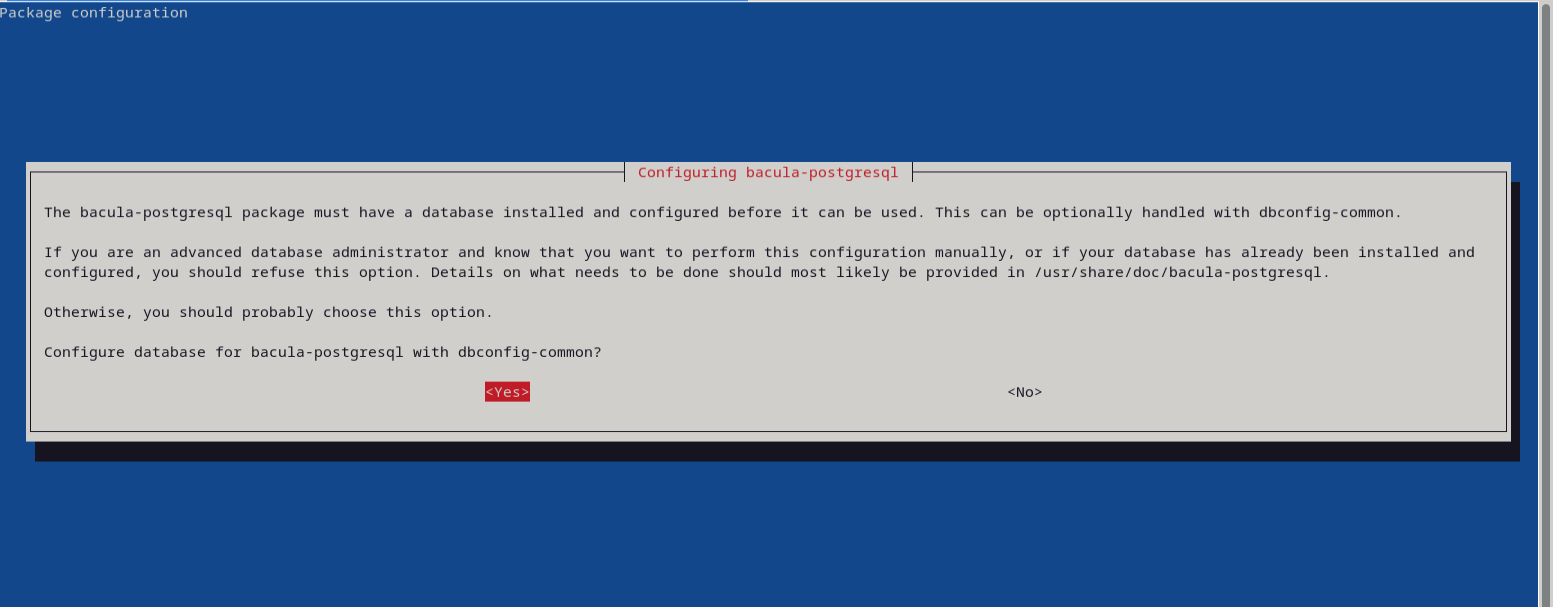
\includegraphics[width=0.5\linewidth]{instalacionBacula/configbaculapostgre.png}
    \caption{Configuración de Bacula con PostgreSQL}
\end{figure}

\textbf{Verificación de la Instalación}\medskip

Finalmente, verificamos que Bacula ha sido instalado correctamente y que todos los componentes necesarios están presentes.

\begin{figure}[H]
    \centering
    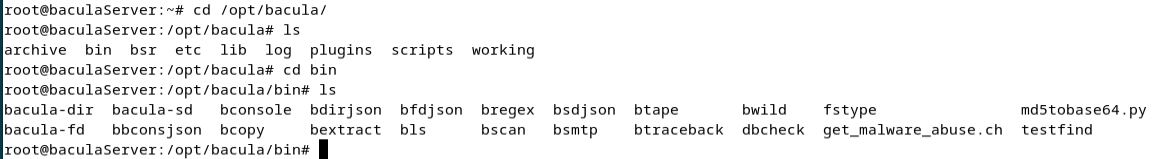
\includegraphics[width=0.5\linewidth]{instalacionBacula/baculadir.png}
    \caption{Verificación de la instalación de Bacula}
\end{figure}

Añadimos al PATH los scripts de Bacula para facilitar la ejecución de comandos:
\begin{verbatim}
export PATH=$PATH:/opt/bacula/bin
\end{verbatim}
